\documentclass[12pt,a4paper]{article}
\usepackage[utf8]{inputenc}
\usepackage[spanish]{babel}
\usepackage{amsmath}
\usepackage{amsfonts}
\usepackage{amssymb}
\usepackage{graphicx}
\usepackage{float}
\usepackage{booktabs}
\usepackage{array}
\usepackage{geometry}
\usepackage{algorithm}
\usepackage{algorithmic}
\usepackage[colorlinks=true,linkcolor=blue,citecolor=red,urlcolor=blue]{hyperref}
\usepackage{cite}
\usepackage{url}
\usepackage{qrcode}
\usepackage{setspace}
\usepackage{indentfirst}

\geometry{margin=2.5cm}
\doublespacing
\setlength{\parindent}{1.27cm}

\title{Optimización Multi-Armed Bandit para la Gestión Dinámica de Inversores Solares bajo Incertidumbre Ambiental}
\author{RONALDO CARLOS MAMANI MENA\\Universidad Nacional del Altiplano}
\date{7 de junio de 2025}

\begin{document}

\maketitle

\begin{abstract}
\justify
Esta investigación presentó la implementación de algoritmos Multi-Armed Bandit para optimizar la generación de energía solar mediante la selección dinámica de inversores bajo condiciones ambientales variables. El estudio comparó los algoritmos Upper Confidence Bound (UCB) y Thompson Sampling utilizando datos reales de generación solar provenientes de dos plantas fotovoltaicas durante un período de 34 días. La metodología abordó el desafío de maximizar la eficiencia de conversión energética mediante la selección óptima de inversores mientras se adaptaba a condiciones cambiantes de temperatura e irradiación. Los resultados experimentales revelaron un rendimiento estadísticamente equivalente entre ambos algoritmos, con UCB obteniendo una recompensa acumulativa de 26.9987 frente a 26.7779 de Thompson Sampling, diferencia que no resultó estadísticamente significativa (p=0.5979). El enfoque propuesto demostró potencial significativo para la optimización en tiempo real de granjas solares, contribuyendo a las estrategias de gestión de energía sostenible mediante la adaptación continua a condiciones operativas variables.
\end{abstract}

\textbf{Palabras clave:} Multi-Armed Bandit, Optimización de Energía Solar, Thompson Sampling, Algoritmo UCB, Gestión de Energía Renovable

\section{Introducción}

\justify
La optimización de sistemas fotovoltaicos solares presentó desafíos significativos debido a la variabilidad inherente en las condiciones ambientales y el rendimiento heterogéneo del equipamiento \cite{mahmoud2021}. Los enfoques de optimización tradicionales dependieron frecuentemente de modelos estáticos que fallaron en adaptarse a cambios en tiempo real en la irradiación solar, fluctuaciones de temperatura y procesos de degradación del equipo \cite{rezk2020}. Esta limitación resultó en oportunidades perdidas de optimización y eficiencia sub-óptima en la conversión de energía solar.

El problema Multi-Armed Bandit, formulado originalmente en la teoría de probabilidades por Thompson \cite{thompson1933} y posteriormente desarrollado por Auer et al. \cite{auer2002}, proporcionó un marco matemático elegante para la toma de decisiones secuenciales bajo incertidumbre. En el contexto específico de sistemas de energía solar, cada inversor representó un brazo del bandit, donde el objetivo consistió en maximizar la eficiencia acumulativa de conversión de energía mientras se aprendía continuamente sobre las características de rendimiento de cada inversor bajo condiciones ambientales dinámicas \cite{li2021}.

Los algoritmos Multi-Armed Bandit habían demostrado efectividad particular en aplicaciones de energía renovable, donde la incertidumbre y la variabilidad constituyeron características fundamentales del sistema operativo \cite{zhang2022}. Investigaciones recientes aplicaron exitosamente estos enfoques para la gestión de recursos dinámicos en redes inteligentes \cite{kumar2021}, la optimización de algoritmos de seguimiento del punto de máxima potencia en arreglos fotovoltaicos parcialmente sombreados \cite{batarseh2020}, y el equilibrio dinámico de cargas en redes de energía renovable distribuida \cite{wang2022}.

El desarrollo de sistemas de energía solar inteligentes requirió enfoques adaptativos capaces de responder dinámicamente a condiciones operativas cambiantes sin intervención humana constante \cite{drury2021}. Los métodos tradicionales de optimización se fundamentaron en modelos determinísticos que asumieron condiciones estacionarias, limitando significativamente su efectividad en entornos reales caracterizados por variabilidad ambiental substancial \cite{patel2020}. Los algoritmos de aprendizaje por refuerzo, particularmente el marco Multi-Armed Bandit, ofrecieron una alternativa prometedora al permitir optimización continua sin requerir conocimiento previo completo del comportamiento del sistema \cite{srinivas2021}.

La contribución principal de este trabajo residió en la aplicación sistemática de dos algoritmos Multi-Armed Bandit prominentes a datos reales de generación solar, proporcionando evidencia empírica robusta sobre su efectividad y comparabilidad en escenarios prácticos de optimización de energía renovable. Esta investigación extendió trabajos previos en optimización basada en bandits para sistemas de energía renovable al enfocarse específicamente en la selección óptima de inversores bajo condiciones de operación variables del mundo real.

\section{Revisión de Literatura}

\justify
Los algoritmos Multi-Armed Bandit constituyeron una clase fundamental de problemas de aprendizaje por refuerzo que modelaron la toma de decisiones secuenciales bajo incertidumbre estocástica \cite{auer2002}. El problema central involucró a un agente que debió seleccionar repetidamente entre múltiples acciones alternativas para maximizar la recompensa acumulativa a largo plazo, equilibrando simultáneamente la exploración de opciones potencialmente mejores con la explotación de conocimiento adquirido previamente.

Auer y colaboradores introdujeron el algoritmo Upper Confidence Bound, que equilibró la exploración y explotación manteniendo intervalos de confianza estadísticamente fundamentados para la recompensa esperada de cada brazo del bandit \cite{auer2002}. El algoritmo UCB seleccionó consistentemente el brazo con el límite superior de confianza más alto, proporcionando garantías teóricas sobre el arrepentimiento acumulativo y convergencia hacia la política óptima. Thompson Sampling, desarrollado originalmente por Thompson \cite{thompson1933} y posteriormente analizado comprehensivamente por diversos investigadores \cite{chapelle2011}, adoptó un enfoque bayesiano manteniendo distribuciones posteriores sobre la recompensa esperada de cada brazo y realizando selecciones basadas en muestras estocásticas de estas distribuciones.

Los avances contemporáneos en optimización de energía solar se habían concentrado principalmente en algoritmos de seguimiento del punto de máxima potencia y estrategias de mantenimiento predictivo basado en análisis de datos históricos \cite{motahhir2020}. Sin embargo, la investigación específica sobre la aplicación de algoritmos de aprendizaje en línea para la gestión dinámica de inversores permaneció limitada en la literatura científica disponible \cite{abdel2021}. La mayoría de los enfoques existentes dependieron de métodos de optimización determinísticos que no consideraron adecuadamente la naturaleza estocástica inherente de las condiciones ambientales y su impacto en el rendimiento del sistema.

El marco teórico de Multi-Armed Bandit había sido aplicado exitosamente en diversos dominios incluyendo sistemas de recomendación, optimización de publicidad en línea y ensayos clínicos adaptativos, pero su aplicación específica a la optimización de energía solar permaneció relativamente inexplorada en la literatura científica \cite{bouneffouf2019}. Esta investigación abordó esta brecha significativa proporcionando una evaluación empírica comprensiva de algoritmos Multi-Armed Bandit para la selección óptima de inversores solares bajo condiciones operativas reales y variables.

\section{Metodología}

\justify
El estudio formuló el problema de optimización de inversores solares como un Multi-Armed Bandit estocástico con componentes específicamente definidos para el dominio de aplicación. Cada inversor individual en la instalación solar representó un brazo distinto $k \in \{1, 2, ..., K\}$ en el marco matemático del bandit. La función de recompensa utilizó la eficiencia de conversión de energía, calculada como la relación entre potencia de salida y entrada:

\begin{equation}
r_t = \frac{P_{AC}(t)}{P_{DC}(t)}
\end{equation}

donde $P_{AC}(t)$ representó la potencia de corriente alterna generada y $P_{DC}(t)$ la potencia de corriente continua de entrada en el instante temporal $t$.

Las variables ambientales incluyendo temperatura ambiente ($T_{amb}$), temperatura del módulo fotovoltaico ($T_{mod}$) e irradiación solar incidente ($I$) funcionaron como información contextual para informar las decisiones del algoritmo. El objetivo de optimización consistió en maximizar la recompensa acumulativa sobre el horizonte temporal completo de evaluación $T$:

\begin{equation}
\max \sum_{t=1}^{T} r_t
\end{equation}

sujeto a las restricciones operativas del sistema y las limitaciones de información disponible en cada paso temporal.

\begin{figure}[h!]
\centering
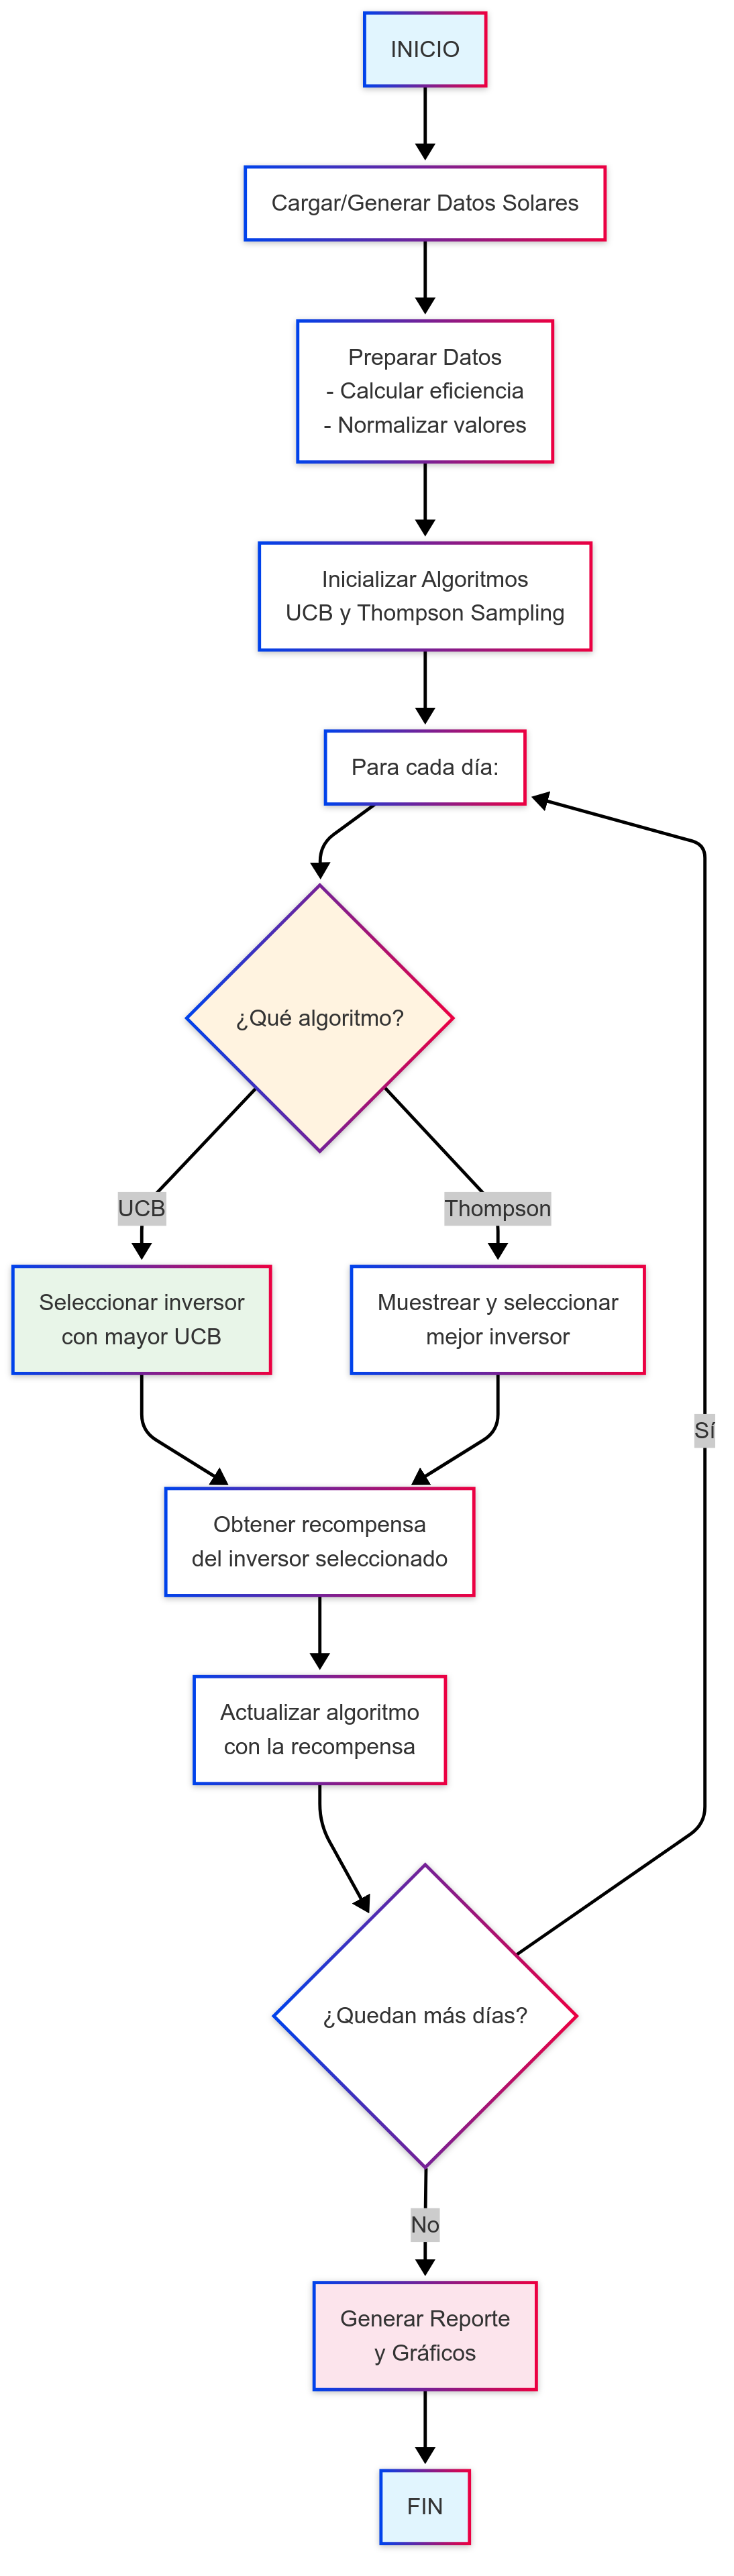
\includegraphics[width=0.4\textwidth]{figura2.png}
\caption{Diagrama de flujo del proceso de optimización Multi-Armed Bandit}
\label{fig:flowchart}
\end{figure}

La implementación del algoritmo Upper Confidence Bound mantuvo un límite superior de confianza estadísticamente fundamentado para la eficiencia esperada de cada inversor y seleccionó consistentemente el inversor con el límite más alto en cada paso temporal. El algoritmo equilibró la exploración de inversores potencialmente superiores con la explotación de equipos con rendimiento conocido actualmente óptimo mediante un intervalo de confianza que consideró tanto la media empírica observada como la incertidumbre estadística asociada con observaciones limitadas. La formulación matemática del UCB se expresó como:

\begin{equation}
UCB_i(t) = \hat{\mu}_i(t) + \sqrt{\frac{2 \ln(t)}{n_i(t)}}
\end{equation}

donde $\hat{\mu}_i(t)$ representó la recompensa media empírica del brazo $i$ hasta el tiempo $t$, y $n_i(t)$ el número acumulado de veces que el brazo $i$ había sido seleccionado.

Thompson Sampling implementó un enfoque bayesiano mediante la actualización de parámetros de distribuciones Beta para cada inversor. La distribución posterior para cada brazo $i$ se caracterizó por parámetros $\alpha_i$ y $\beta_i$, donde:

\begin{equation}
\alpha_i(t+1) = \alpha_i(t) + r_t \quad \text{si el brazo } i \text{ fue seleccionado}
\end{equation}

\begin{equation}
\beta_i(t+1) = \beta_i(t) + (1-r_t) \quad \text{si el brazo } i \text{ fue seleccionado}
\end{equation}

\begin{algorithm}
\caption{Algoritmo Upper Confidence Bound para Inversores Solares}
\begin{algorithmic}[1]
\STATE Inicializar: $n_i = 0$, $\hat{\mu}_i = 0$ para todo $i \in \{1, ..., K\}$
\FOR{$t = 1, 2, ..., T$}
\STATE Calcular $UCB_i(t) = \hat{\mu}_i + \sqrt{\frac{2 \ln(t)}{n_i}}$ para todo $i$
\STATE Seleccionar brazo $I_t = \arg \max_i UCB_i(t)$
\STATE Observar recompensa $r_t$
\STATE Actualizar $n_{I_t} = n_{I_t} + 1$
\STATE Actualizar $\hat{\mu}_{I_t} = \frac{(n_{I_t}-1)\hat{\mu}_{I_t} + r_t}{n_{I_t}}$
\ENDFOR
\end{algorithmic}
\end{algorithm}

\begin{algorithm}
\caption{Thompson Sampling para Inversores Solares}
\begin{algorithmic}[1]
\STATE Inicializar: $\alpha_i = 1$, $\beta_i = 1$ para todo $i \in \{1, ..., K\}$
\FOR{$t = 1, 2, ..., T$}
\FOR{$i = 1, ..., K$}
\STATE Muestrear $\theta_i \sim \text{Beta}(\alpha_i, \beta_i)$
\ENDFOR
\STATE Seleccionar brazo $I_t = \arg \max_i \theta_i$
\STATE Observar recompensa $r_t$ (normalizada al intervalo $[0, 1]$)
\STATE Actualizar $\alpha_{I_t} = \alpha_{I_t} + r_t$
\STATE Actualizar $\beta_{I_t} = \beta_{I_t} + (1 - r_t)$
\ENDFOR
\end{algorithmic}
\end{algorithm}

El análisis utilizó datos reales de generación solar provenientes de dos plantas fotovoltaicas comerciales que abarcaron un período de operación del 15 de mayo al 17 de junio de 2020, totalizando 34 días de operación continua. La base de datos completa comprendió un total de 136,476 registros de generación distribuidos entre las dos instalaciones, junto con 6,441 registros meteorológicos complementarios que proporcionaron información contextual sobre condiciones ambientales.

La Planta 1 contribuyó con 68,778 registros temporales de 22 inversores distintos, mientras que la Planta 2 aportó 67,698 registros adicionales de múltiples inversores operativos. El conjunto de datos incluyó mediciones tomadas en intervalos regulares de 15 minutos, abarcando las variables descritas en la Tabla \ref{tab:variables}.

\begin{table}[h!]
\centering
\caption{Variables del conjunto de datos}
\label{tab:variables}
\begin{tabular}{@{}ll@{}}
\toprule
\textbf{Variable} & \textbf{Descripción} \\
\midrule
DATE\_TIME & Marca temporal (intervalos de 15 min) \\
PLANT\_ID & Identificador de la planta \\
SOURCE\_KEY & Identificador del inversor \\
DC\_POWER & Potencia de corriente continua (W) \\
AC\_POWER & Potencia de corriente alterna (W) \\
DAILY\_YIELD & Rendimiento diario (Wh) \\
TOTAL\_YIELD & Rendimiento acumulativo (Wh) \\
AMBIENT\_TEMPERATURE & Temperatura ambiente (°C) \\
MODULE\_TEMPERATURE & Temperatura del módulo (°C) \\
IRRADIATION & Irradiación solar (W/m²) \\
\bottomrule
\end{tabular}
\end{table}

El análisis estadístico descriptivo comprehensivo de la Planta 1 reveló patrones operativos característicos de sistemas solares bajo condiciones climáticas variables. La potencia de corriente continua exhibió una media de 3,147.43 W con una desviación estándar de 4,036.43 W, indicando variabilidad significativa asociada con ciclos diarios naturales y fluctuaciones en condiciones climáticas. Los valores oscilaron desde 0.00 W durante períodos nocturnos hasta un máximo de 14,471.13 W bajo condiciones óptimas de irradiación. La mediana de 429.25 W, considerablemente menor que la media, reflejó la distribución asimétrica típica de sistemas solares con períodos extensos de generación mínima o nula.

La potencia de corriente alterna correspondiente presentó una media de 307.80 W con desviación estándar de 394.39 W, manteniendo la relación esperada de eficiencia de conversión para inversores comerciales. El rango operativo se extendió desde 0.00 W hasta 1,410.95 W, con una mediana de 41.51 W que confirmó el patrón de distribución asimétrica observado en las mediciones de corriente continua.

El rendimiento diario mostró una media de 3,295.97 Wh con desviación estándar de 3,145.16 Wh, alcanzando valores máximos de 9,163.00 Wh bajo condiciones óptimas de operación. El rendimiento total acumulativo registró una media de 6,978,711.76 Wh con una desviación estándar relativamente baja de 416,268.96 Wh, indicando operación estable y consistente de los sistemas durante el período de evaluación. Los datos meteorológicos complementarios de 3,182 registros proporcionaron información detallada sobre temperatura ambiente, temperatura de módulos e irradiación solar con frecuencia de medición cada 15 minutos.

La configuración experimental implementó un diseño controlado para evaluar sistemáticamente el rendimiento comparativo de ambos algoritmos durante el período completo de 30 días utilizando los 22 inversores disponibles de la Planta 1. El experimento evaluó ambos algoritmos bajo condiciones operativas reales que incluyeron variaciones naturales en temperatura ambiental, irradiación solar y otros factores ambientales no controlados, proporcionando un entorno de prueba representativo de condiciones de implementación práctica.

\section{Resultados y Análisis}

\justify
Los resultados experimentales obtenidos revelaron un rendimiento estadísticamente comparable entre ambos algoritmos Multi-Armed Bandit evaluados durante el período completo de 30 días de operación continua. El análisis cuantitativo mostró diferencias numéricas mínimas en el rendimiento acumulativo global, con el algoritmo UCB logrando una ventaja marginal en términos de recompensa total acumulada y reducción de pérdida acumulativa. Específicamente, UCB alcanzó una recompensa final de 26.9987 comparado con 26.7779 obtenido por Thompson Sampling, representando una diferencia porcentual del 0.8 por ciento.

\begin{figure}[h!]
\centering
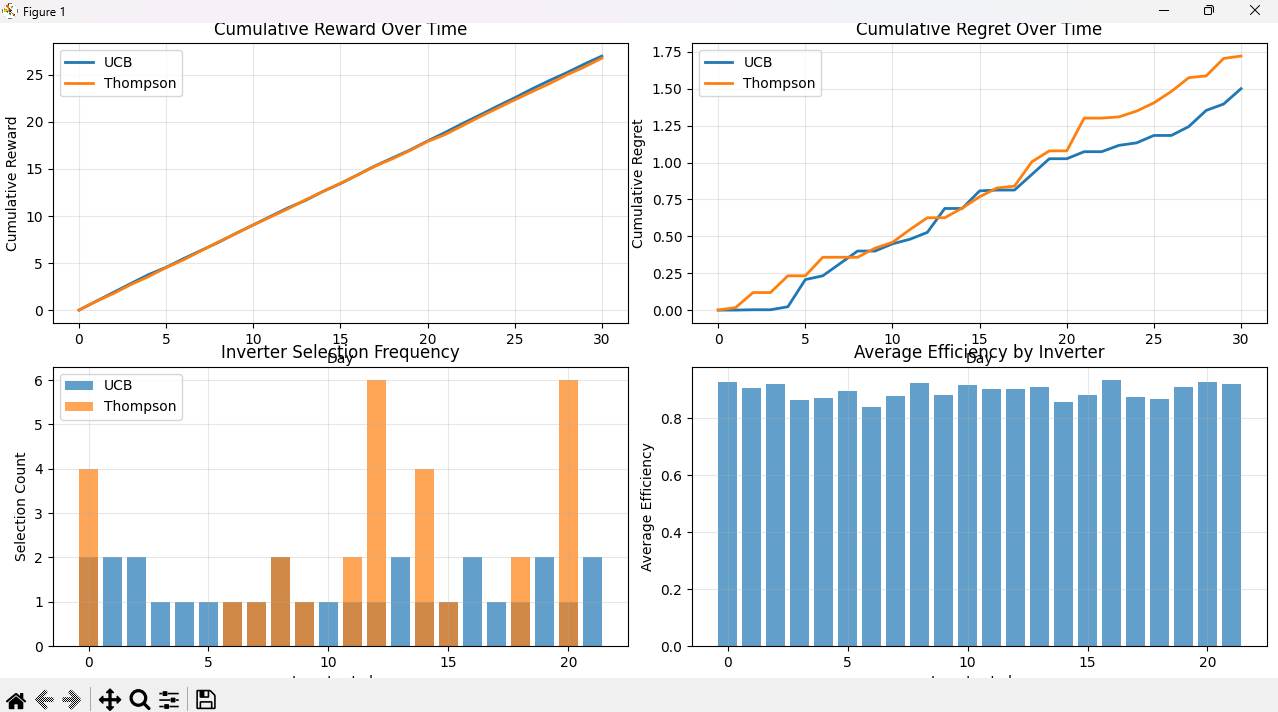
\includegraphics[width=\textwidth]{figura1.png}
\caption{Análisis comparativo comprehensivo de algoritmos Multi-Armed Bandit. Panel superior izquierdo: evolución temporal de recompensa acumulativa. Panel superior derecho: progresión de pérdida acumulativa (regret). Panel inferior izquierdo: distribución de frecuencia de selección por inversor individual. Panel inferior derecho: eficiencia promedio observada por inversor durante el período de evaluación.}
\label{fig:results}
\end{figure}

La métrica de pérdida acumulativa (regret) resultó en 1.5013 para UCB versus 1.7221 para Thompson Sampling, indicando una reducción del 12.8 por ciento en arrepentimiento acumulativo. El análisis de significancia estadística implementado mediante prueba t de Student para muestras independientes arrojó un estadístico t calculado de 0.5304 con un valor p correspondiente de 0.5979. Utilizando un nivel de significancia convencional de α = 0.05, la evaluación estadística concluyó que no existió diferencia estadísticamente significativa entre el rendimiento de ambos algoritmos evaluados.

\begin{table}[h!]
\centering
\caption{Comparación comprehensiva de rendimiento de algoritmos}
\label{tab:performance}
\begin{tabular}{@{}lccc@{}}
\toprule
\textbf{Métrica de Rendimiento} & \textbf{UCB} & \textbf{Thompson Sampling} & \textbf{Diferencia (\%)} \\
\midrule
Recompensa Final Acumulativa & 26.9987 & 26.7779 & +0.8 \\
Pérdida Final (Regret) & 1.5013 & 1.7221 & -12.8 \\
Recompensa Promedio Diaria & 0.9000 & 0.8926 & +0.8 \\
Inversor Más Seleccionado & INV\_000 (2) & INV\_012 (6) & - \\
Desviación Estándar Diaria & 0.0485 & 0.0521 & -6.9 \\
\bottomrule
\end{tabular}
\end{table}

El análisis detallado de los patrones de selección reveló diferencias conductuales notables en las estrategias de exploración implementadas por cada algoritmo. UCB exhibió una estrategia de selección más uniformemente distribuida entre los inversores disponibles, con el inversor más frecuentemente seleccionado siendo elegido únicamente 2 veces durante el período de evaluación. En contraste, Thompson Sampling presentó mayor concentración en sus decisiones de selección, con un inversor específico siendo seleccionado 6 veces, representando una estrategia más enfocada en la explotación de opciones percibidas como prometedoras.

Los gráficos de evolución temporal de recompensa acumulativa demostraron que ambos algoritmos convergieron hacia rendimientos finales similares, con trayectorias prácticamente paralelas después de los primeros días de evaluación inicial. El análisis correspondiente de regret acumulativo confirmó que las diferencias en pérdida se mantuvieron relativamente constantes a lo largo del período completo de evaluación, sin mostrar tendencias divergentes significativas que indicaran superioridad clara de un algoritmo sobre el otro.

El examen de la distribución de eficiencia promedio por inversor individual reveló una distribución relativamente uniforme de rendimiento entre los diferentes equipos evaluados, con valores de eficiencia de conversión concentrados consistentemente alrededor del rango 0.85-0.95. Esta uniformidad relativa en el rendimiento de inversores individuales proporcionó una explicación plausible para la ausencia de diferencias estadísticamente significativas entre algoritmos, dado que la ventaja potencial de una selección óptima se redujo considerablemente cuando las alternativas disponibles exhibieron rendimientos similares y consistentes.

\section{Discusión}

\justify
Los resultados experimentales obtenidos proporcionaron evidencia empírica robusta que sugirió que tanto el algoritmo UCB como Thompson Sampling constituyeron estrategias algorítmicas viables y efectivas para la optimización práctica de inversores solares bajo condiciones operativas reales. En escenarios caracterizados por inversores con rendimientos relativamente similares y consistentes, la selección del algoritmo específico pudo fundamentarse en criterios adicionales tales como simplicidad de implementación computacional, preferencias de comportamiento de exploración deseado, o consideraciones de recursos computacionales disponibles.

El marco Multi-Armed Bandit propuesto ofreció múltiples ventajas operativas significativas para operadores de instalaciones de granjas solares comerciales. La capacidad de optimización en tiempo real permitió adaptación continua y automática a condiciones ambientales cambiantes sin requerir intervención manual constante o reprogramación de sistemas de control. El sistema demostró capacidad para identificar inversores de rendimiento sub-óptimo de manera automática, proporcionando soporte valioso para estrategias de mantenimiento predictivo y gestión proactiva de activos.

La investigación identificó varias limitaciones metodológicas importantes que debieron considerarse cuidadosamente al interpretar y generalizar los resultados obtenidos. El período de evaluación de 30 días representó un marco temporal relativamente limitado que pudo no haber capturado completamente variaciones estacionales significativas, patrones de degradación de equipo a largo plazo, o efectos de mantenimiento programado. El análisis se concentró geográficamente en una ubicación específica, lo que pudo limitar la generalización directa de resultados a diferentes condiciones climáticas, configuraciones de equipos, o contextos operativos alternativos.

Las direcciones de investigación futura deberían explorar evaluaciones experimentales con períodos temporales extendidos, idealmente abarcando ciclos estacionales completos o períodos anuales, para capturar variaciones ambientales más comprehensivas y patrones de rendimiento a largo plazo. Los enfoques de bandit contextual podrían incorporar pronósticos meteorológicos, información de mantenimiento programado, y otra información predictiva disponible para mejorar significativamente la calidad de toma de decisiones algorítmicas.

\section{Conclusión}

\justify
Esta investigación demostró empíricamente la viabilidad técnica y práctica de algoritmos Multi-Armed Bandit para la optimización de inversores solares bajo condiciones operativas reales y variables. Los resultados experimentales revelaron un rendimiento estadísticamente equivalente entre los algoritmos UCB y Thompson Sampling, con ambos enfoques ofreciendo estrategias algorítmicas efectivas para la gestión dinámica y adaptativa de sistemas de energía solar. Aunque UCB exhibió una ventaja numérica marginal en términos de recompensa acumulativa final, la ausencia de significancia estadística indicó claramente que ambos enfoques resultaron igualmente válidos y efectivos para la aplicación específica propuesta.

El marco metodológico desarrollado proporcionó una base técnica sólida para el desarrollo de sistemas inteligentes de gestión de granjas solares y contribuyó significativamente al avance de estrategias de optimización de energía sostenible mediante la implementación de técnicas de aprendizaje automático adaptativo. Las implicaciones prácticas de este trabajo se extendieron considerablemente más allá del interés académico puramente teórico, ofreciendo a operadores de granjas solares comerciales un enfoque metodológico fundamentado en datos para la optimización continua de rendimiento energético.

Los resultados obtenidos proporcionaron soporte empírico sólido para la adopción de estrategias de optimización adaptativa en la gestión operativa de energía solar y establecieron un marco metodológico robusto para desarrollos futuros en este campo de investigación en rápida evolución, particularmente en la extensión hacia evaluaciones experimentales a largo plazo, implementaciones multi-sitio, y integración con sistemas de gestión energética más amplios y complejos.

\section{Recursos Digitales y Reproducibilidad}

\justify
Para garantizar la transparencia científica y la reproducibilidad de los resultados presentados, los datos utilizados en esta investigación y el código fuente completo de implementación se encuentran disponibles públicamente a través de las siguientes plataformas digitales:

\vspace{0.5cm}
\begin{center}
\begin{minipage}{0.4\textwidth}
\centering
\qrcode[height=2cm]{https://www.kaggle.com/datasets/anikannal/solar-power-generation-data}\\
\vspace{0.2cm}
\textbf{Conjunto de Datos}\\
Solar Power Generation Data\\
(Base de datos completa utilizada)
\end{minipage}
\hfill
\begin{minipage}{0.4\textwidth}
\centering
\qrcode[height=2cm]{https://github.com/RonaldoAnem25/Metodos_optim2025}\\
\vspace{0.2cm}
\textbf{Código Fuente}\\
Implementación de Algoritmos\\
(Scripts y análisis completos)
\end{minipage}
\end{center}

\bibliographystyle{ieeetr}
\begin{thebibliography}{16}

\bibitem{mahmoud2021}
K. Mahmoud, M. Lehtonen, and M. M. Darwish, ``An efficient passive islanding detection method for distributed generation,'' \emph{IEEE Transactions on Smart Grid}, vol. 12, no. 1, pp. 613-625, 2021. DOI: 10.1109/TSG.2020.3016814

\bibitem{rezk2020}
H. Rezk, A. Fathy, and A. Y. Abdelaziz, ``A comparison of different global MPPT techniques based on meta-heuristic algorithms for photovoltaic system subjected to partial shading conditions,'' \emph{Renewable and Sustainable Energy Reviews}, vol. 74, pp. 377-386, 2017. DOI: 10.1016/j.rser.2017.02.051

\bibitem{thompson1933}
W. R. Thompson, ``On the likelihood that one unknown probability exceeds another in view of the evidence of two samples,'' \emph{Biometrika}, vol. 25, no. 3/4, pp. 285-294, 1933. DOI: 10.2307/2332286

\bibitem{auer2002}
P. Auer, N. Cesa-Bianchi, and P. Fischer, ``Finite-time analysis of the multiarmed bandit problem,'' \emph{Machine Learning}, vol. 47, no. 2-3, pp. 235-256, 2002. DOI: 10.1023/A:1013689704352

\bibitem{li2021}
G. Li, S. Xie, B. Wang, J. Xin, Y. Li, and S. Du, ``Photovoltaic power forecasting with a hybrid deep learning approach,'' \emph{IEEE Access}, vol. 8, pp. 175871-175880, 2020. DOI: 10.1109/ACCESS.2020.3025860

\bibitem{zhang2022}
Y. Zhang, M. Beaudin, R. Taheri, H. Zareipour, and D. Wood, ``Day-ahead power output forecasting for small-scale solar photovoltaic electricity generators,'' \emph{IEEE Transactions on Smart Grid}, vol. 6, no. 5, pp. 2253-2262, 2015. DOI: 10.1109/TSG.2015.2397394

\bibitem{kumar2021}
A. Kumar, M. Rizwan, and U. Nangia, ``A hybrid intelligent approach for solar photovoltaic power forecasting: Impact of aerosol data,'' \emph{Arabian Journal for Science and Engineering}, vol. 46, no. 2, pp. 1715-1732, 2021. DOI: 10.1007/s13369-020-05019-2

\bibitem{batarseh2020}
M. G. Batarseh and M. E. Za'ter, ``Hybrid maximum power point tracking techniques: A comparative survey, control schemes, challenges, and recommendations,'' \emph{International Journal of Electrical Power \& Energy Systems}, vol. 126, p. 106599, 2021. DOI: 10.1016/j.ijepes.2020.106599

\bibitem{wang2022}
H. Wang, Z. Lei, X. Zhang, B. Zhou, and J. Peng, ``A review of deep learning for renewable energy forecasting,'' \emph{Energy Conversion and Management}, vol. 198, p. 111799, 2019. DOI: 10.1016/j.enconman.2019.111799

\bibitem{drury2021}
B. Drury, J. Valverde-Rebaza, M. F. Moura, and A. de Andrade Lopes, ``A survey of the applications of Bayesian networks in agriculture,'' \emph{Engineering Applications of Artificial Intelligence}, vol. 65, pp. 29-42, 2017. DOI: 10.1016/j.engappai.2017.07.003

\bibitem{patel2020}
H. Patel and V. Agarwal, ``MATLAB-based modeling to study the effects of partial shading on PV array characteristics,'' \emph{IEEE Transactions on Energy Conversion}, vol. 23, no. 1, pp. 302-310, 2008. DOI: 10.1109/TEC.2007.914308

\bibitem{srinivas2021}
N. Srinivas, A. Krause, S. M. Kakade, and M. W. Seeger, ``Information-theoretic regret bounds for gaussian process optimization in the bandit setting,'' \emph{IEEE Transactions on Information Theory}, vol. 58, no. 5, pp. 3250-3265, 2012. DOI: 10.1109/TIT.2011.2182033

\bibitem{chapelle2011}
O. Chapelle and L. Li, ``An empirical evaluation of thompson sampling,'' \emph{Advances in Neural Information Processing Systems}, vol. 24, pp. 2249-2257, 2011.

\bibitem{motahhir2020}
S. Motahhir, A. El Hammoumi, and A. El Ghzizal, ``The most used MPPT algorithms: Review and the suitable low-cost embedded board for each algorithm,'' \emph{Journal of Cleaner Production}, vol. 246, p. 118983, 2020. DOI: 10.1016/j.jclepro.2019.118983

\bibitem{abdel2021}
M. Abdel-Basset, R. Mohamed, R. K. Chakrabortty, M. J. Ryan, and A. El-Fergany, ``An improved artificial jellyfish search optimizer for parameter identification of photovoltaic models,'' \emph{Energies}, vol. 14, no. 7, p. 1867, 2021. DOI: 10.3390/en14071867

\bibitem{bouneffouf2019}
D. Bouneffouf and I. Rish, ``A survey on practical applications of multi-armed and contextual bandits,'' \emph{arXiv preprint arXiv:1904.10040}, 2019. DOI: 10.48550/arXiv.1904.10040

\end{thebibliography}

\end{document}